Following the requisites enumerated in \autoref{chap:Biosensors}, a sensor based on the measure of impedance seems to be ideal. Impedimetric sensors are generally simple and affordable, portable, robust, and permit measurements on the fly and digital storage to memory. \par

Impedance sensors can be separated in two categories: resistive sensors and capacitive sensors (see \autoref{app:CapacitanceBiosensors} for a short literature review of Capacitance biosensors, which was also published as a section in the soon-to-be-published "A Comprehensive Review of Advances in Electrochemical Biosensors for Microbial Monitoring" by Seyedeh Nazila Hosseini. Some parameters are notable when designing such sensors, such as the detection principle, the resolution, delays, response time, dynamic range, excitation frequency range, sensor and electrodes size, linearity, number of channels, precision, input waveform, and power dissipation \cite{Carminati2017}. The change in impedance can be caused by a variation of the materials resistivity, dielectric constant, or geometry. The resistivity and dielectric constant depend on the mobility and quantity of charge carriers in the material. Electrons in metals and semiconductors, photoconductor, and ions in electrolytic solutions are examples of change to the number of charge carrier, whereas temperature variations can instancy the change to the mobility of charge carrier \cite{Carminati2017}. An ideal sensor would maximize the time response, the dynamic range, the excitation frequency range, the linearity, and the precision of the measurements; while minimizing the delay times, the size of the sensor and electrodes, and the power dissipation. \par

An impedance is defined from the complex Ohm's law \cite{leHuy2004circuits} based on the ratio of a voltage signal to a current signal : 
\begin{equation}
   Z(j\omega) = \frac{V_{in}(j\omega)}{I_{out}(j\omega)} = \frac{V_{out}(j\omega)}{I_{in}(j\omega)} = \frac{V_m}{I_m} \times e^{-j\phi} = \lvert Z \rvert e^{-j\phi} = \Re(Z) +j \times \Im(Z)
   \label{eq:ImpedanceEIS}
\end{equation}
Where $Z$ is the impedance, $V$ is the applied (or measured) voltage, $I$ is the measured (or applied) current, $\phi$ is the phase difference between the voltage and current, $\omega$ is the angular frequency, and $j$ is the imaginary unit value. \autoref{fig:VoltageCurrent} describes some of these parameters. \par
\begin{figure}[h]
    \centering
    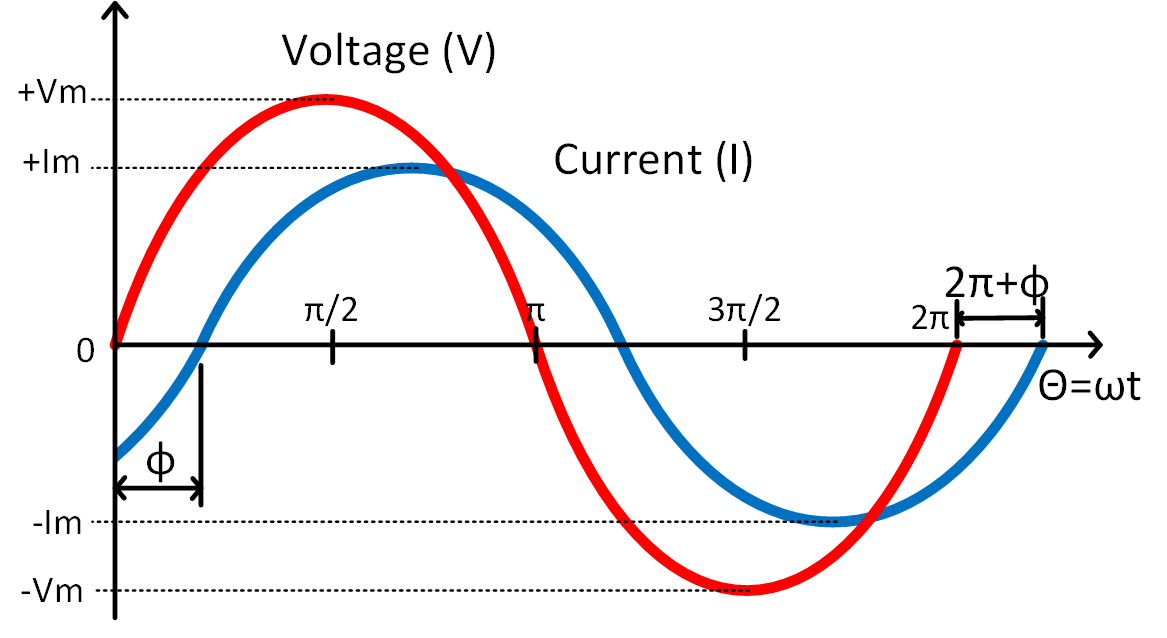
\includegraphics[width=0.7\textwidth]{VoltageCurrent}
    \caption{Current and voltage sinewaves.}
    \label{fig:VoltageCurrent}
\end{figure}

When considering current and voltage signals constituted only of sinusoids of the same frequency, an analytical representation can be used to simplify the mathematics involved and represent the values as phasors. Phasors are complex representations and can thus be represented in a 2-dimensional plane as a function of their real and imaginary components for rectangular forms, or magnitude and phase for polar forms (see \autoref{fig:ComplexImpedance}). The Real part of the impedance is assimilated to a resistance $R$ value, which is the component of an impedance responsable for power-dissipation. The Imaginary part of the impedance is assimilated to a Reactance $X$ value, which affects the signal without dissipating power. The magnitude $\lvert Z \rvert$ and phase $\phi$ of the impedance can be retrieved from the Real and Imaginary components using equation \autoref{eq:Magnitude} and \autoref{eq:Phase}. \par
\begin{equation}
    \label{eq:Magnitude}
    \lvert Z \rvert = \sqrt{\Re(Z)^2+\Im(Z)^2)}
\end{equation}
\begin{equation}
    \label{eq:Phase}
   \phi = \atan(\frac{\Im(Z)}{\Re(Z)})
\end{equation}
\begin{figure}[h]
    \centering
    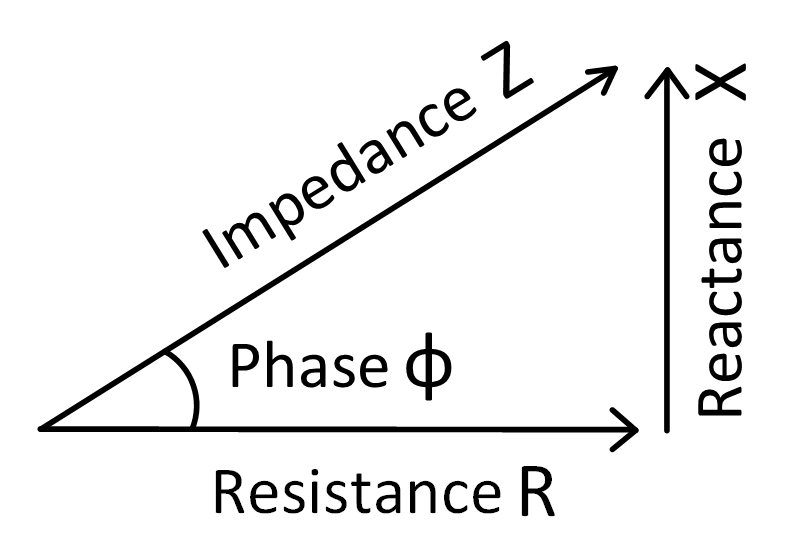
\includegraphics[width=0.4\textwidth]{ComplexImpedance}
    \caption{Impedance represented in a complex 2-d plane}
    \label{fig:ComplexImpedance}
\end{figure}